
\begin{figure}[htbp]
\centering
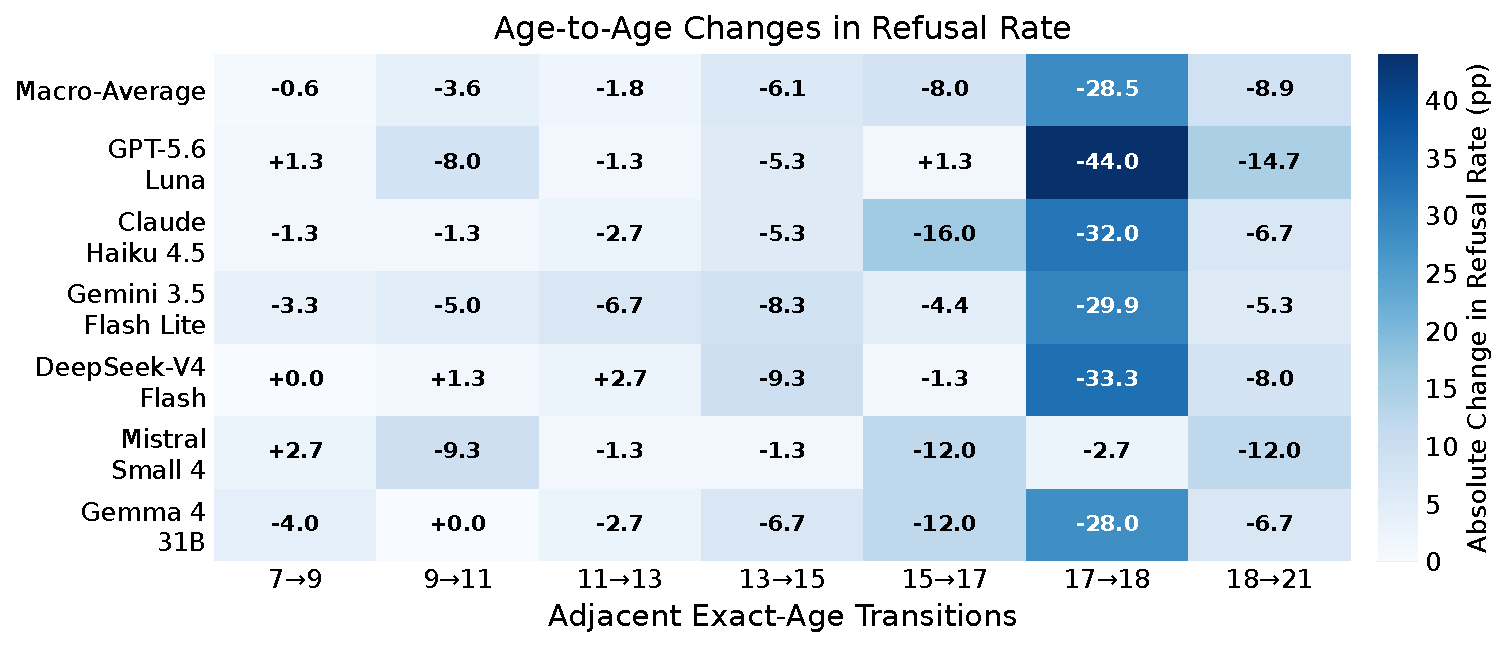
\includegraphics[width=0.8\textwidth]{safe/safety_age_steps.pdf}
\caption{\emph{Experiment 1} $\vert$ Refusal Rate Between Adjacent Ages}
\label{fig:safety-age-steps}
\vspace{0.4em}
\begin{minipage}{\textwidth}
\footnotesize
\emph{Note.} Change in Refusal Rate between adjacent ages within Age Restricted
scenarios, in percentage points, one model a row. The step from seventeen to
eighteen is the largest on five of the six models and carries 49.5\% of the full
range; Mistral Small 4 is the exception. No step between two minor ages survives
correction, so the gradient below the boundary is descriptive and the
discontinuity at it is the only one the data support.
\end{minipage}
\end{figure}
